\documentclass{article}
\usepackage{graphicx} % Required for inserting images
\usepackage{booktabs}
\usepackage{amssymb}
\usepackage[figuresleft]{rotating}
% --- ISARC Page Layout & Margins ---
\usepackage[a4paper, top=3.5cm, bottom=3.5cm, left=2.5cm, right=2.0cm]{geometry}
\graphicspath{{images/}}

% If you are setting up the full two-column paper layout:
\setlength{\columnsep}{0.5cm}
\title{Multi-Robot Evaluation Table}
\author{Jose Pablo Araya Castillo}
\date{August 2026}

\begin{document}


\begin{sidewaystable}
    

\centering
\caption{Viability of Panel Assembly based on Robotic Cell Configurations}
\label{tab:cell_configurations}
\renewcommand{\arraystretch}{1.5} % Adds breathing room for the multiline text
% p{4.5cm} forces the first column to wrap text. 
% The ten 'c's center the 10 panel columns.
\setlength{\tabcolsep}{3pt}
\begin{tabular}{@{} p{4.0cm} | c c c c c c c c c @{}}
\toprule
\hline

% ROW 1: Panel IDs
\textbf{Cell \newline Configuration} & 
\textbf{1E-02} & 
\textbf{1E-04} & 
\textbf{1E-11} & 
\textbf{2E-01} & 
\textbf{2E-07} & 
\textbf{2E-26} & 
\textbf{3E-11} & 
\textbf{3E-19} & 
\textbf{3E-20} \\

% ROW 2: Panel Images
&
\raisebox{-.5\height}{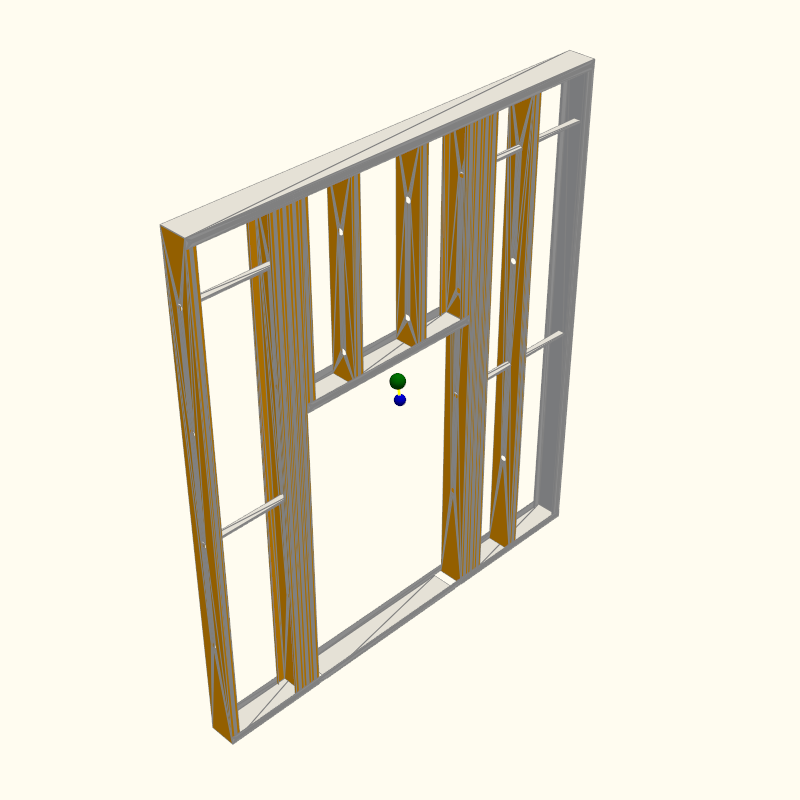
\includegraphics[width=0.07\textwidth]{1E-2_Render (1).png}} & 
\raisebox{-.5\height}{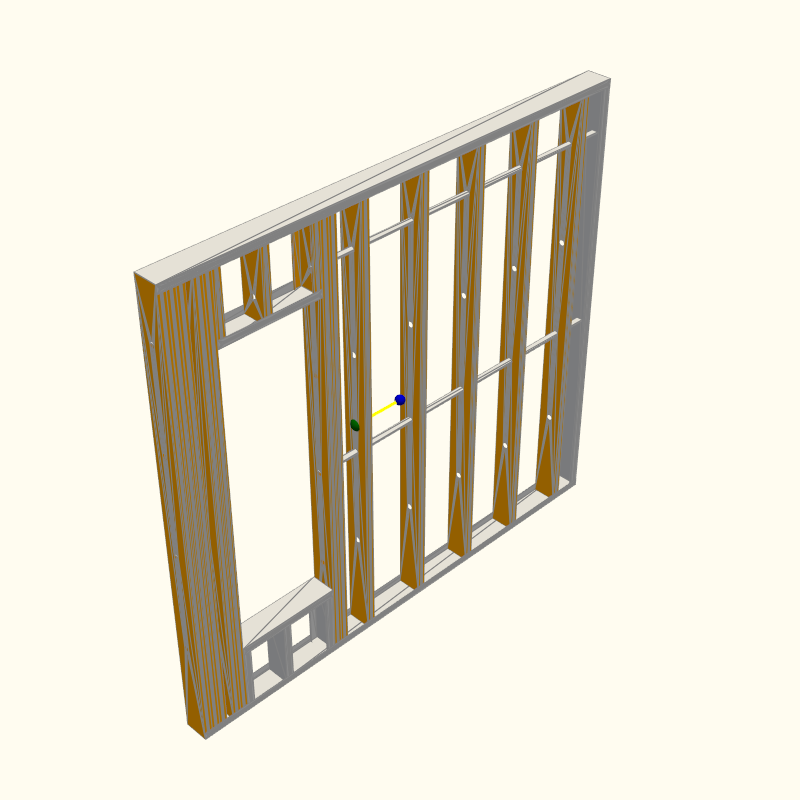
\includegraphics[width=0.07\textwidth]{1E-4_Render.png}} & 
\raisebox{-.5\height}{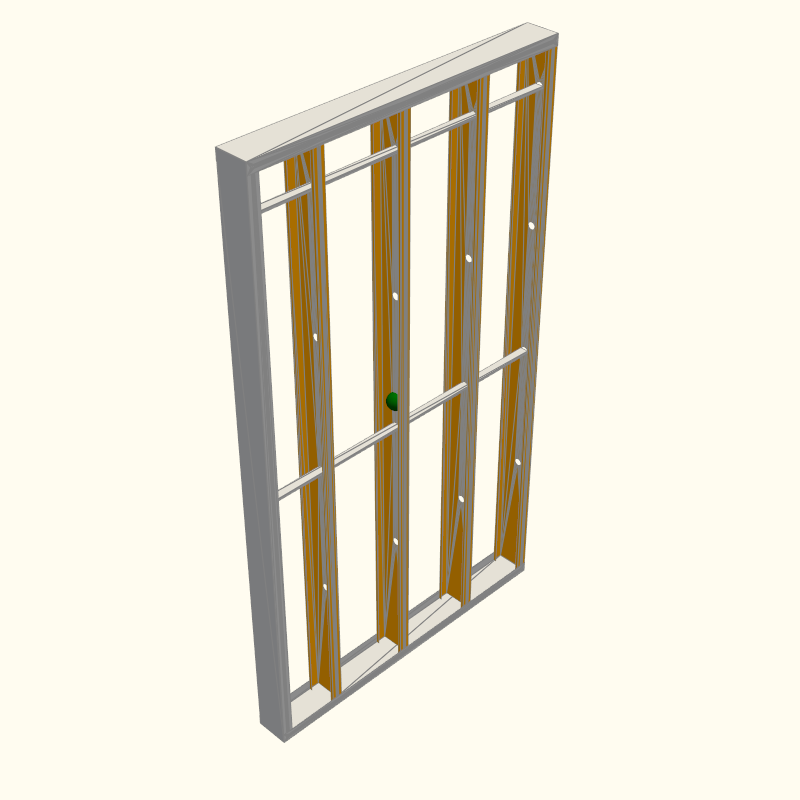
\includegraphics[width=0.07\textwidth]{1E-11_Render.png}} & 
\raisebox{-.5\height}{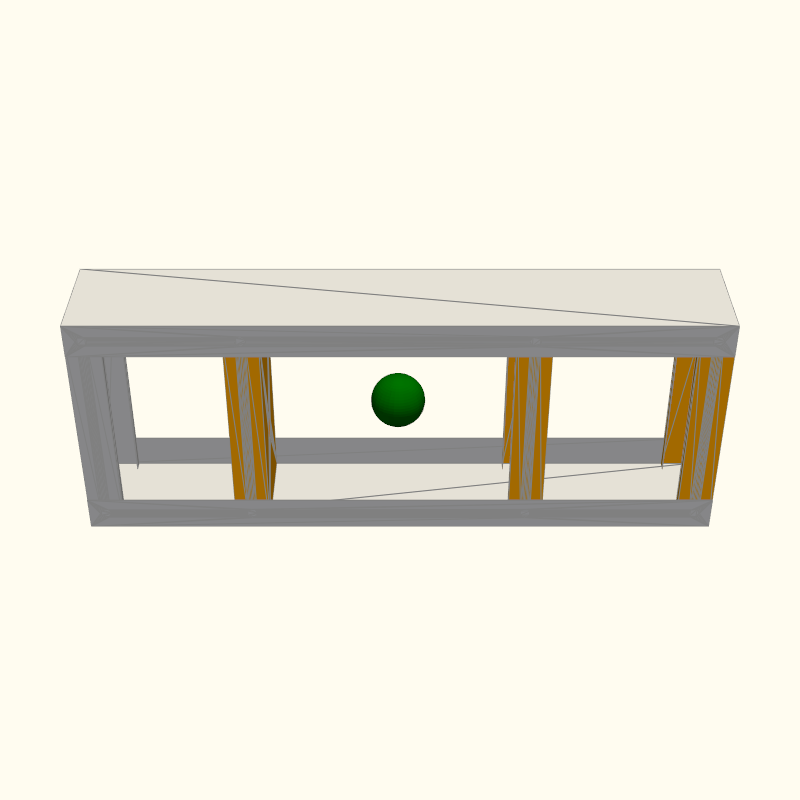
\includegraphics[width=0.07\textwidth]{2E-1_Render.png}} & 
\raisebox{-.5\height}{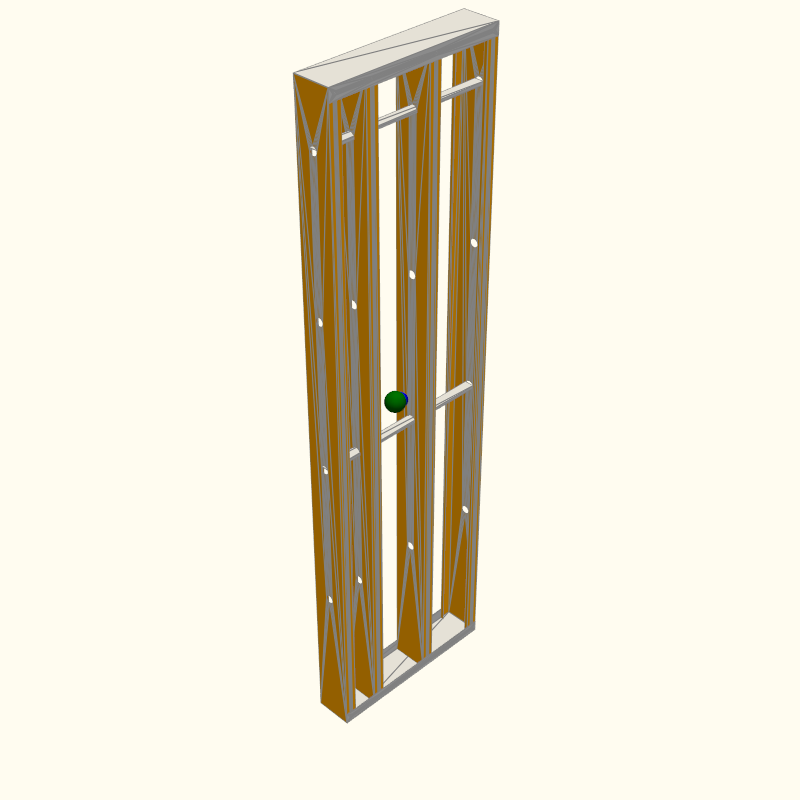
\includegraphics[width=0.07\textwidth]{2E-7_Render.png}} & 
\raisebox{-.5\height}{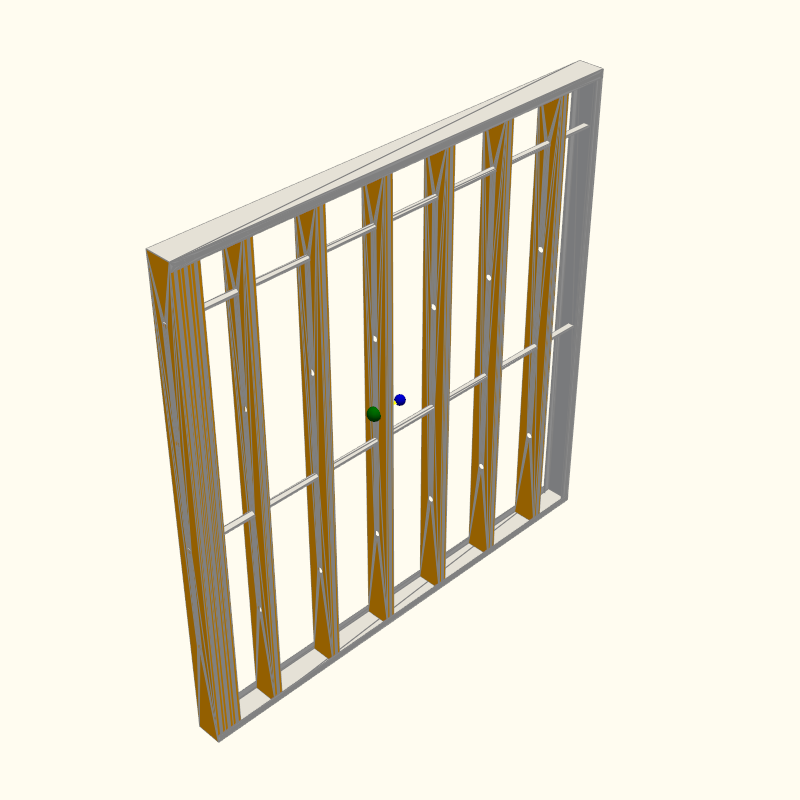
\includegraphics[width=0.07\textwidth]{2E-26_Render.png}} & 
\raisebox{-.5\height}{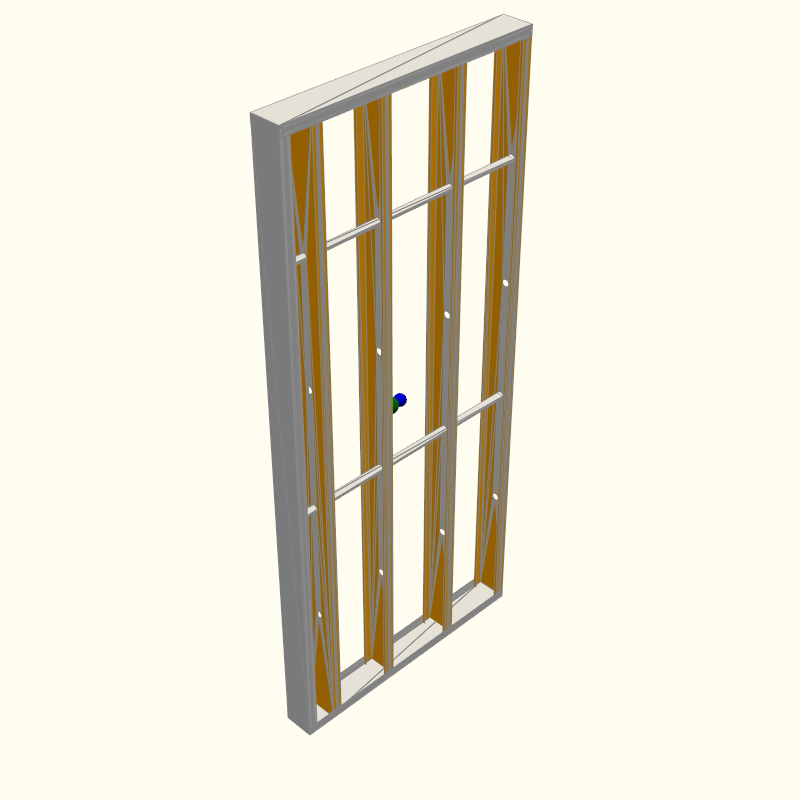
\includegraphics[width=0.07\textwidth]{3E-11 (1)_Render.png}} & 
\raisebox{-.5\height}{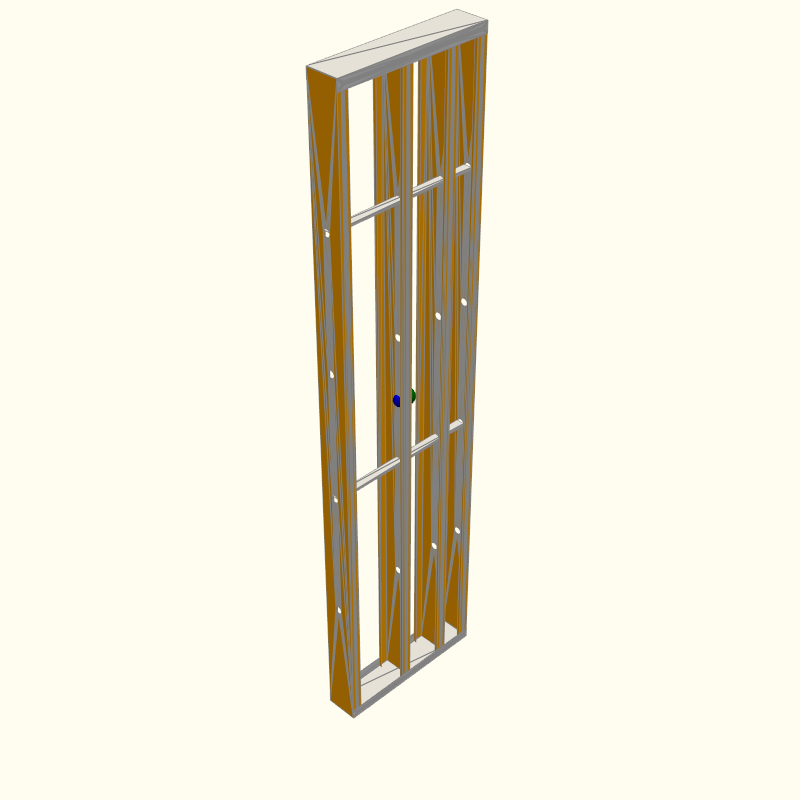
\includegraphics[width=0.07\textwidth]{3E-19_Render.png}} & 
\raisebox{-.5\height}{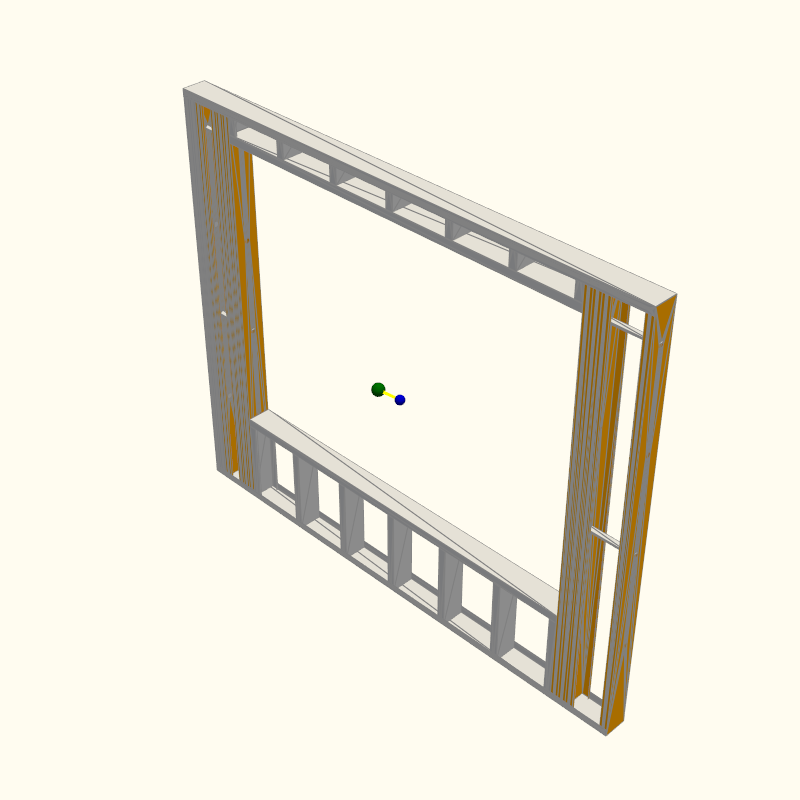
\includegraphics[width=0.07\textwidth]{3E-20_Render.png}} \\

% ROW 3
ABB IRB 2600-20/1.65 & 
$\times$ & 
$\times$ & 
$\times$ & 
$\checkmark$ & 
$\times$ & 
$\times$ & 
$\times$ & 
$\times$ & 
$\times$ \\

% ROW 4
ABB IRB 2600-20/1.65 \newline + IRBT 2005 Linear Unit & 
$\times$ & 
$\times$ & 
$\checkmark$ & 
$\checkmark$ & 
$\checkmark$ & 
$\times$ & 
$\checkmark$ & 
$\checkmark$ & 
$\times$ \\

% ROW 5
ABB IRB 2600-20/1.65 \newline + Dobot CR10 & 
$\times$ & 
$\times$ & 
$\checkmark$ & 
$\checkmark$ & 
$\checkmark$ & 
$\times$ & 
$\times$ & 
$\times$ & 
$\times$ \\

% ROW 6
ABB IRB 2600-20/1.65 \newline + IRBT 2005 \newline + Dobot CR10 & 
$\checkmark$ & 
$\checkmark$ & 
$\checkmark$ & 
$\checkmark$ & 
$\checkmark$ & 
$\checkmark$ & 
$\checkmark$ & 
$\checkmark$ & 
$\checkmark$ \\

% ROW 7
DOBOT CR10 (Helper) & 
$\times$ & 
$\times$ & 
$\times$ & 
$\checkmark$ & 
$\times$ & 
$\times$ & 
$\times$ & 
$\times$ & 
$\times$ \\

% ROW 8
KUKA KR 250 R2700-2 & 
$\times$ & 
$\times$ & 
$\checkmark$ & 
$\checkmark$ & 
$\checkmark$ & 
$\times$ & 
$\times$ & 
$\times$ & 
$\times$ \\

% ROW 9
KUKA KR 250 R2700-2 \newline + Dobot CR10 & 
$\checkmark$ & 
$\times$ & 
$\checkmark$ & 
$\checkmark$ & 
$\checkmark$ & 
$\checkmark$ & 
$\checkmark$ & 
$\checkmark$ & 
$\checkmark$ \\

\bottomrule
\end{tabular}
\end{sidewaystable}

\end{document}